\documentclass{beamer}
\usepackage{xcolor}
\usepackage{natbib} % package to organize literature
\usepackage{multicol}
\usepackage{booktabs}
\usepackage{wasysym} % additional symbols
\usepackage{graphicx} % to include graphics, gifs
\usepackage{color} % add colored text
\usepackage{lmodern} % to fix font size error, might be problematic with math symbols
\usepackage{array}

\usetheme{Frankfurt}
\usecolortheme{beaver}
\setbeamertemplate{footline}
{
  \leavevmode%
  \hbox{%
  \begin{beamercolorbox}[wd=.3\paperwidth,ht=2.25ex,dp=1ex,center]{author in head/foot}%
    \usebeamerfont{author in head/foot}\insertshortauthor \hspace{1em} (\insertshortinstitute)
  \end{beamercolorbox}%
  \begin{beamercolorbox}[wd=.4\paperwidth,ht=2.25ex,dp=1ex,center]{title in head/foot}%
    \usebeamerfont{title in head/foot}\insertshorttitle
  \end{beamercolorbox}%
  \begin{beamercolorbox}[wd=.3\paperwidth,ht=2.25ex,dp=1ex,right]{author in head/foot}%
    \usebeamerfont{author in head/foot}\insertdate \hspace{2em}
    \insertframenumber{} / \inserttotalframenumber\hspace*{1em}
  \end{beamercolorbox}}%
  \vskip0pt%
}
%\definecolor{beamer@sbred}{rgb}{0.65,0.15,0.18}
\definecolor{beamer@sbred}{rgb}{0.22,0.22,0.66}
\setbeamercolor{title}{fg=beamer@sbred,bg=black!5}
\setbeamercolor{structure}{fg=beamer@sbred}
\setbeamercolor{frametitle}{fg=beamer@sbred}
\setbeamercolor{palette primary}{fg=beamer@sbred,bg=black!10}
\setbeamercolor{palette secondary}{fg=beamer@sbred}
\setbeamercolor{palette tertiary}{bg=beamer@sbred}
\setbeamercolor{palette quaternary}{fg=white,bg=beamer@sbred}
\setbeamertemplate{itemize items}[default]
\setbeamertemplate{enumerate items}[default]
\setbeamersize{text margin left=1em,text margin right=1em}
\DeclareTextFontCommand{\emph}{\color{beamer@sbred}}

\author[Kraft \& DeScioli]{Patrick Kraft \and Peter DeScioli}
\institute[Stony Brook]{Center for Behavioral Political Economy}
\title[Voter Utilities and Majority Voting]{How the Nature of Political Preferences Shapes the Efficiency of Majority Rule Voting}
\date{October 16, 2014}
\titlegraphic{\includegraphics[width=4cm]{/data/Dropbox/1-src/logos/logo_bk.pdf}}

\begin{document}
\frame{\titlepage}
%\footnotesize


\section{Introduction}

\subsection{}
\begin{frame}%[allowframebreaks]
\frametitle{Questions}
\begin{itemize}
\item Is the majority rule \emph{efficient}?
\item How does its efficiency depend on how we \emph{conceptualize} individual preferences and utilities?
\end{itemize}
\end{frame}

\subsection{}
\begin{frame}%[allowframebreaks]
\frametitle{Background}
\begin{itemize}
\item Condorcet Jury Theorem
\begin{itemize}
  \item majority rule is efficient
  \item information aggregation
\end{itemize}
\item What about conflicting preferences?
\end{itemize}
\end{frame}

\begin{frame}%[allowframebreaks]
\frametitle{Inefficient Majorities}
\begin{table}[c]
  \caption{Example for Inefficient Majorities}
  \begin{center}
    \begin{tabular}{lcc}
    \hline
    \textbf{Voter} & \textbf{Candidate A} & \textbf{Candidate B} \\
    \hline
       Alice & \$0 & \$100 \\
       Betty & \$20 & \$10 \\
       Carol & \$10 & \$0 \\
    \hline
    \end{tabular}
  \end{center}
\end{table}
\end{frame}

\begin{frame}%[allowframebreaks]
\frametitle{Adding a third candidate candidate}
\begin{table}[c]
  \caption{Example for Cyclic Preferences}
  \begin{center}
    \begin{tabular}{lccc}
    \hline
    \textbf{Voter} & \textbf{Candidate A} & \textbf{Candidate B} & \textbf{Candidate C} \\
    \hline
       Alice & \$0 & \$100 & \$10 \\
       Betty & \$20 & \$10 & \$0 \\
       Carol & \$10 & \$0 & \$20 \\
    \hline
    \end{tabular}
  \end{center}
\end{table}
\end{frame}

\subsection{}
\begin{frame}%[allowframebreaks]
\frametitle{Voting, Ideal Points, and Utilities I}
\begin{itemize}
  \item \emph{Spatial theory of voting} \citep[e.g.][]{downs1957economic,westholm1997distance}:
  \begin{itemize}
     \item common policy / ideological dimension
     \item utilities determined by relative \emph{proximity}
   \end{itemize}
  \end{itemize}
  $$U_i^\text{cand} = -(X_i - X^\text{cand})^2$$
\end{frame}

\begin{frame}%[allowframebreaks]
\frametitle{Voting, Ideal Points, and Utilities II}
\begin{table}[c]
  \caption{Example for Cyclic Preferences}
  \begin{center}
    \begin{tabular}{lccc}
    \hline
    \textbf{Voter} & \textbf{Candidate A} & \textbf{Candidate B} & \textbf{Candidate C} \\
    \hline
       Alice & \$0 & \$100 & \$10 \\
       Betty & \$20 & \$10 & \$0 \\
       Carol & \$10 & \$0 & \$20 \\
    \hline
    \end{tabular}
  \end{center}
  \begin{figure}[b]\centering
      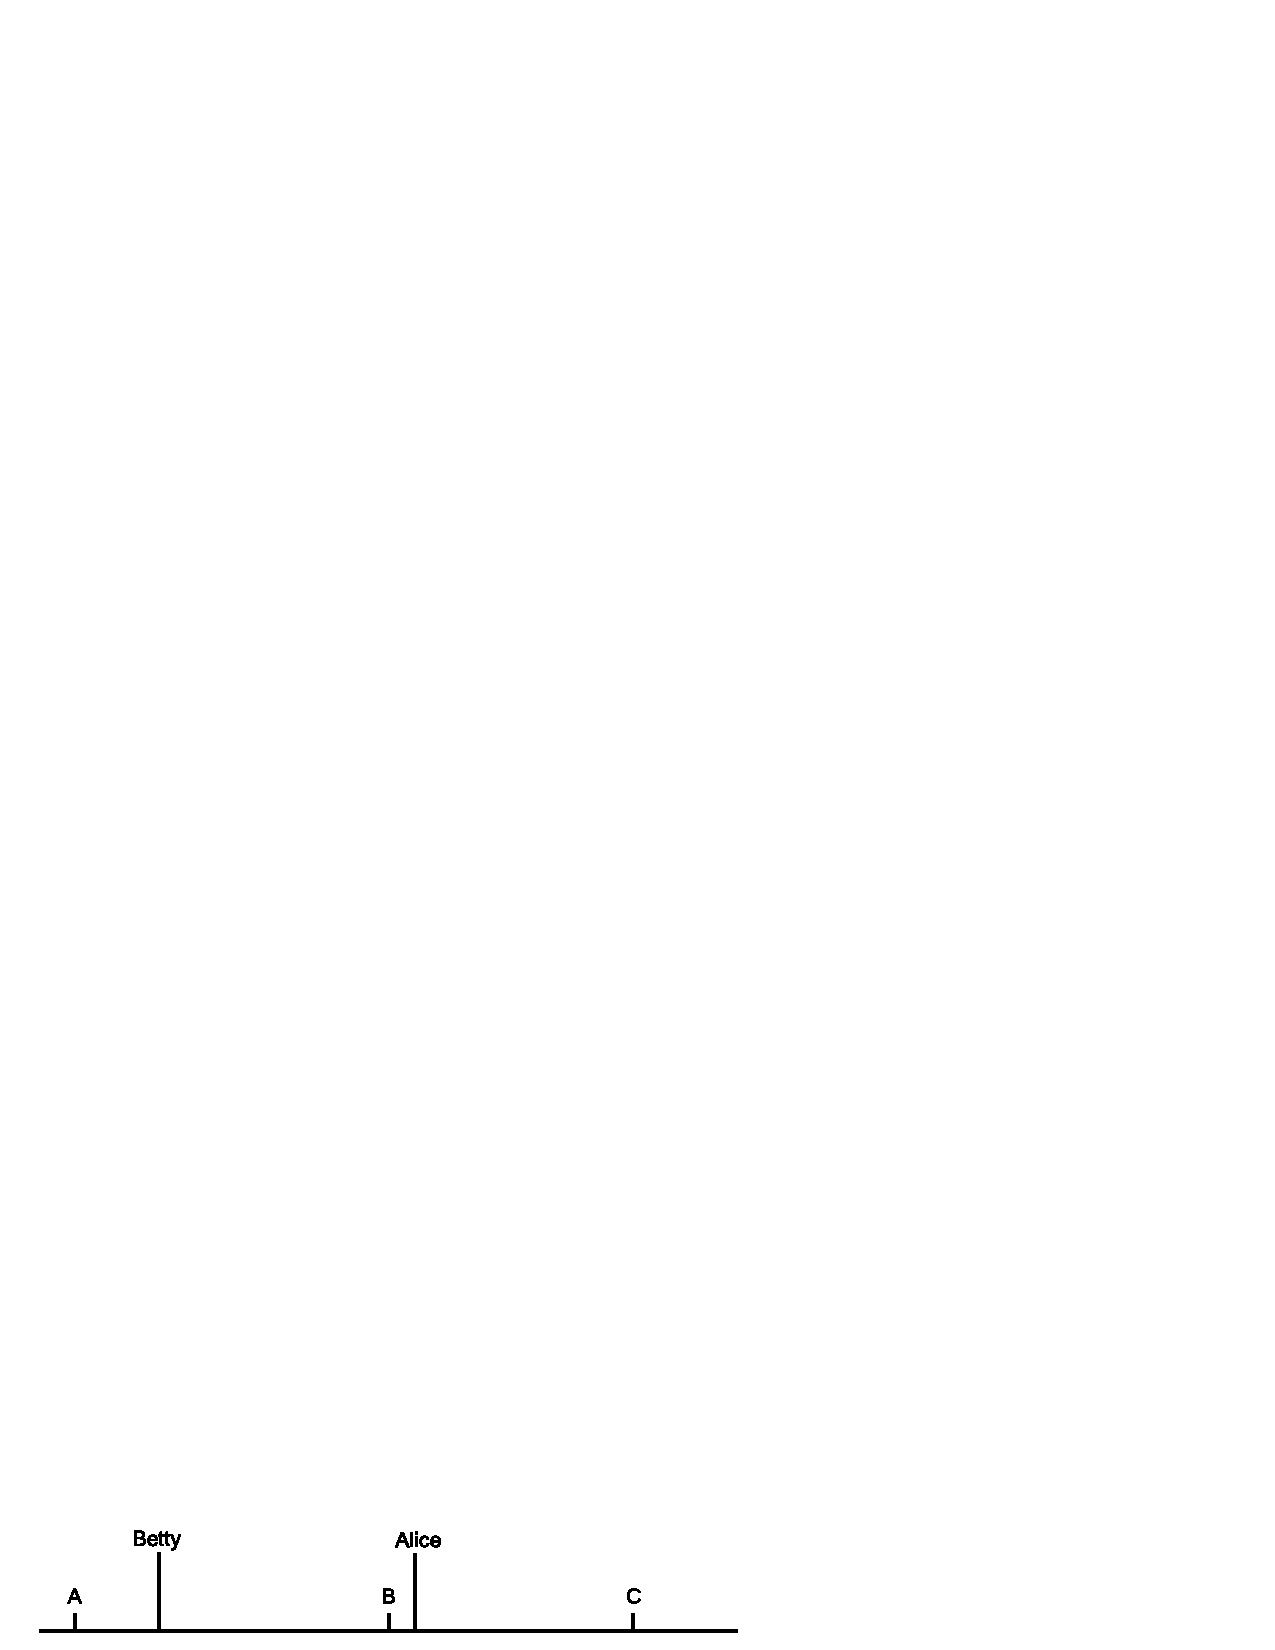
\includegraphics[width=.8\textwidth]{plot.pdf}
  \end{figure}
\end{table}
\end{frame}

\subsection{}
\begin{frame}%[allowframbreaks]
  \frametitle{Back to the initial question}
  \begin{itemize}
  \item Formal voting models: \emph{common policy space}
  \item \emph{Other factors} influence preferences and utilities, e.g. candidate traits and appearance \citep[e.g.][]{hayes2005candidate,todorov2005inferences}
\item \emph{Question:} How can relaxing assumptions of issue-based utilities alter our conclusions about the efficiency of voting rules?
\end{itemize}
\end{frame}


\section{Simulation Results}
\subsection{}
\begin{frame}%[allowframebreaks]
  \frametitle{Simulation Scenarios}
  \begin{itemize}
    \item Overview:
    \begin{itemize}
      \item Number of \emph{voters} in each election: 2000
      \item Number of \emph{candidates} in each election: 2
      \item Number of \emph{simulations} for each scenario: 1000
      \item Individual \emph{utilities} based on ideal points or directly simulated from distributions; voters vote for the candidate that maximizes their utility
      \item \emph{Goal:} investigate the \emph{efficiency} of majority voting under varying assumptions about voter preferences
    \end{itemize}
    \item Conceptualization of efficiency:
    \begin{itemize}
      \item Does the election result \emph{maximize the aggregated utilities} for all voters?
      \item $ \sum_i U_i^{W} > \sum_i U_i^{L} $
    \end{itemize}
  \end{itemize}
\end{frame}

\subsection{}
\begin{frame}%[allowframebreaks]
  \frametitle{First comparison of ideal points and normal utilities I}
  \begin{figure}[ht]\centering
    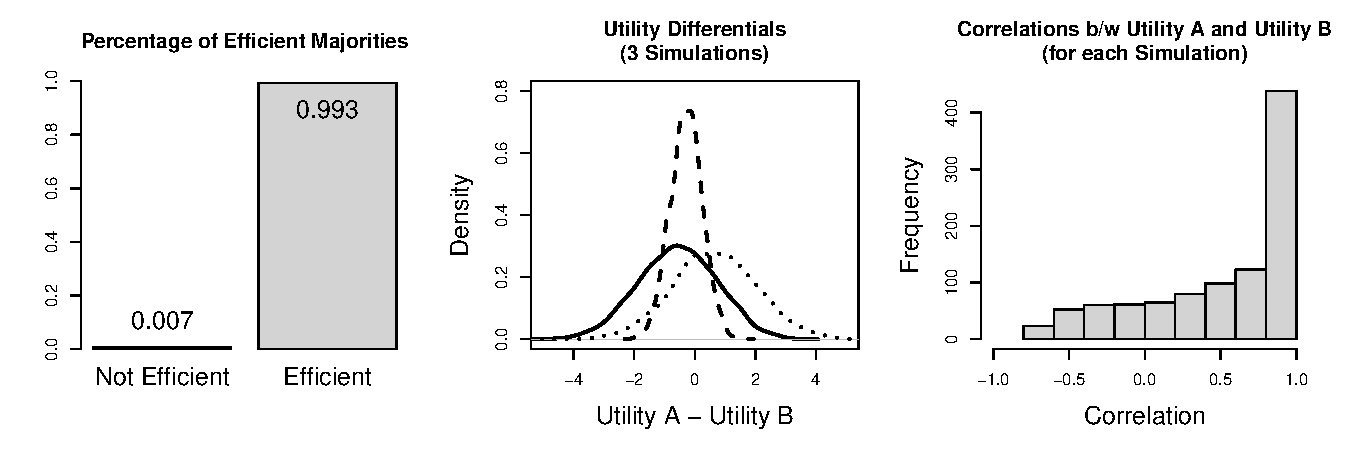
\includegraphics[width=\textwidth]{../calc/fig/s1a.pdf}
    \caption{Normally distributed ideal points}
  \end{figure}
  $$X_i,X_a,X_b \sim \mathcal{N}(\mu=0,\sigma^2=1)$$
  $$U^a_i = -(X_i - X_a)^2 \hspace{1cm} U^b_i = -(X_i - X_b)^2$$
\end{frame}
\begin{frame}%[allowframebreaks]
  \frametitle{First comparison of ideal points and normal utilities II}
  \begin{figure}[ht]\centering
    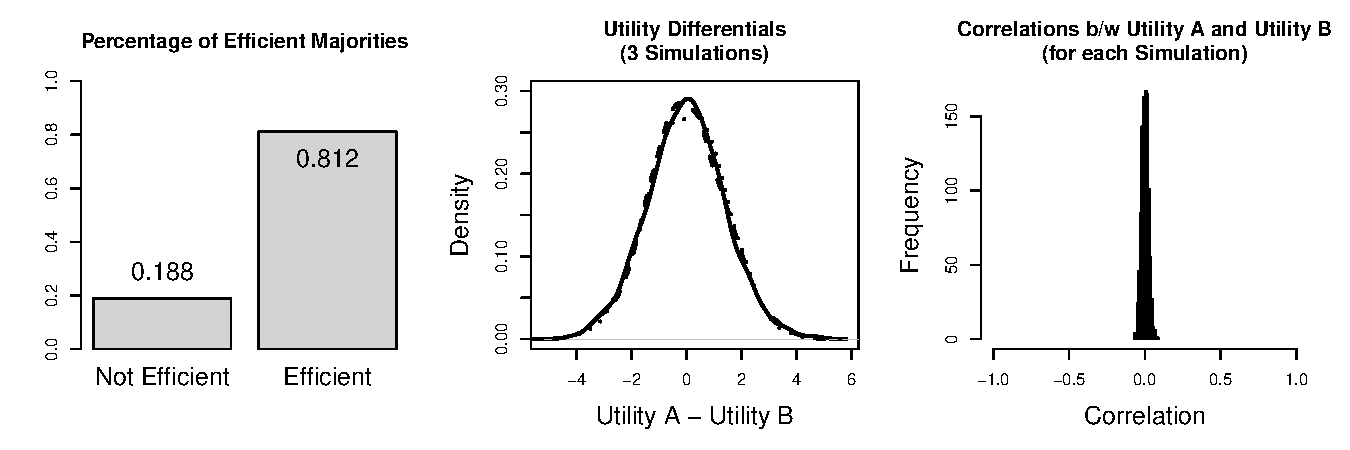
\includegraphics[width=\textwidth]{../calc/fig/s1b.pdf}
    \caption{Independent normal utilities}
  \end{figure}
  $$U^a_i,U^b_i \sim \mathcal{N}(\mu=0,\sigma^2=1)$$
\end{frame}

\subsection{}
\begin{frame}%[allowframebreaks]
  \frametitle{Investigating the effect of correlated utilities I}
  \begin{figure}[ht]\centering
    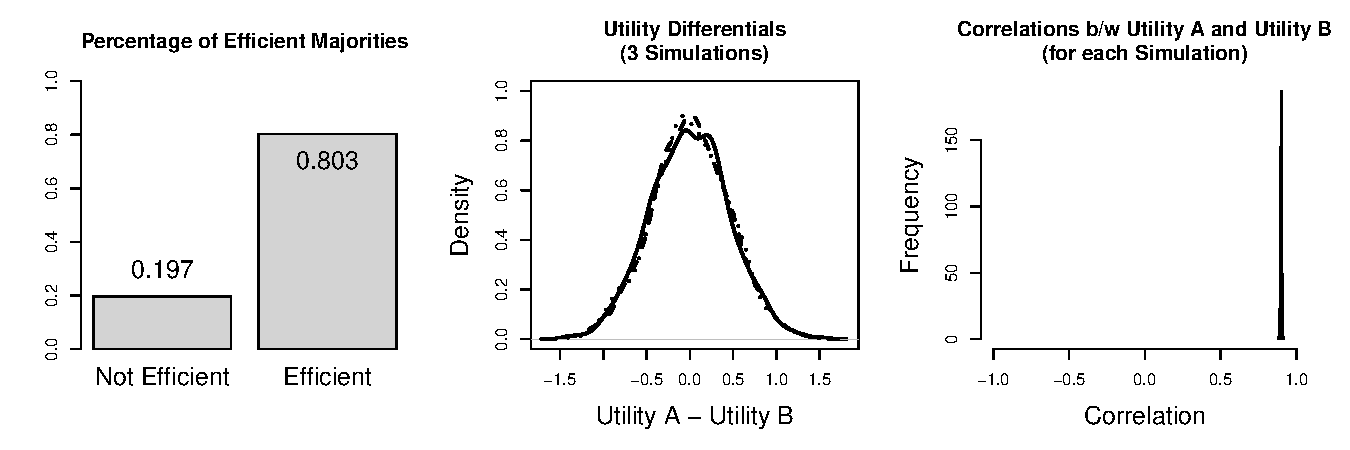
\includegraphics[width=\textwidth]{../calc/fig/s2a.pdf}
    \caption{Positively correlated normal utilities}
  \end{figure}
  $$U_a,U_b \sim \mathcal{N}\left(
    \mathbf{\mu}=\begin{pmatrix}0 \\ 0\end{pmatrix},
    \mathbf{\Sigma}=\begin{pmatrix}1 & 0.9 \\ 0.9 & 1\end{pmatrix}
    \right)$$
\end{frame}
\begin{frame}%[allowframebreaks]
  \frametitle{Investigating the effect of correlated utilities II}
  \begin{figure}[ht]\centering
    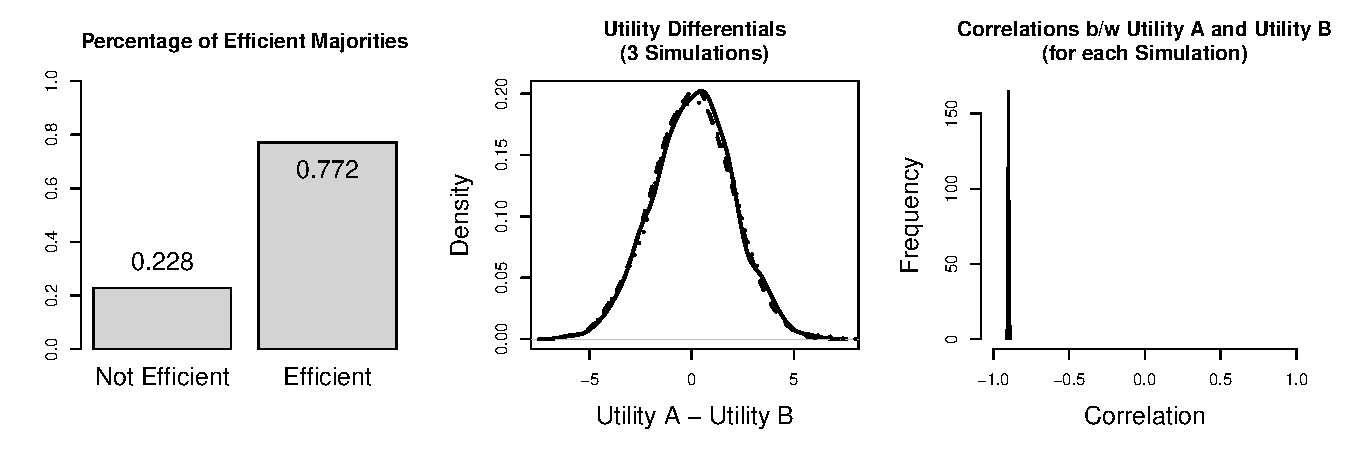
\includegraphics[width=\textwidth]{../calc/fig/s2b.pdf}
    \caption{Negatively correlated normal utilities}
  \end{figure}
  $$ U_a, U_b \sim \mathcal{N}\left(
    \mathbf{\mu}=\begin{pmatrix}0 \\ 0\end{pmatrix},
    \mathbf{\Sigma}=\begin{pmatrix}1 & -0.9 \\ -0.9 & 1\end{pmatrix}
    \right)$$
\end{frame}

\subsection{}
\begin{frame}%[allowframebreaks]
  \frametitle{Inefficiencies for varying mean differences in utilities I}
  \begin{figure}[ht]\centering
    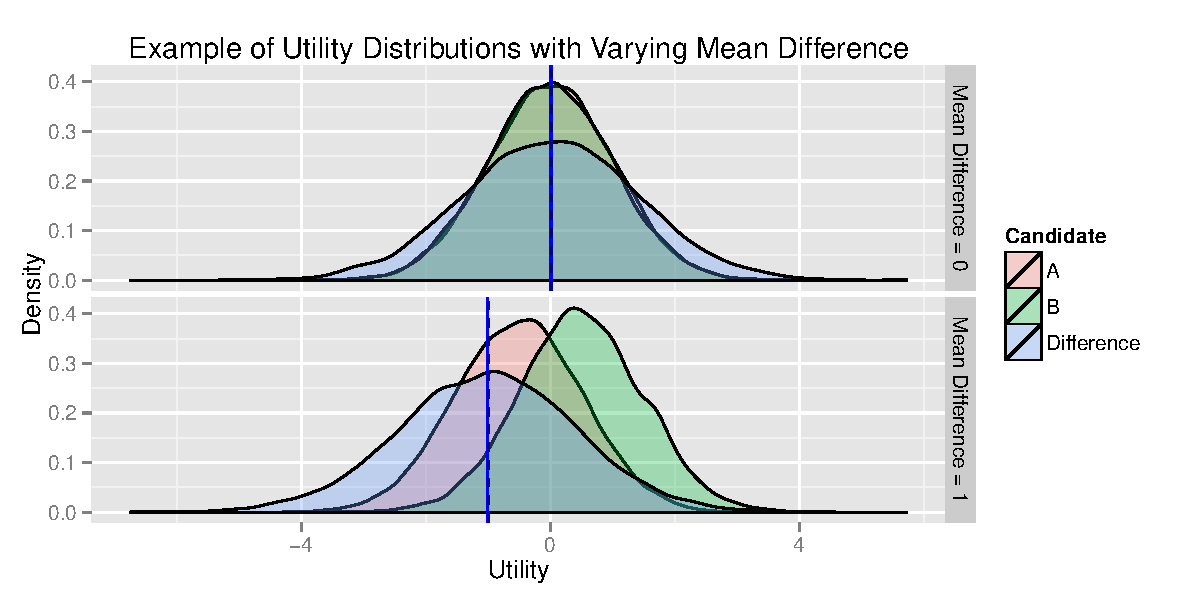
\includegraphics[height=.7\textheight]{../calc/fig/s3a.pdf}
  \end{figure}
  $$U^a_i \sim \mathcal{N}(\mu=0,\sigma^2=1) \hspace{1cm}
  U^b_i \sim \mathcal{N}(\mu=0+\epsilon,\sigma^2=1)$$
\end{frame}
\begin{frame}%[allowframebreaks]
  \frametitle{Inefficiencies for varying mean differences in utilities II}
  \begin{figure}[ht]\centering
    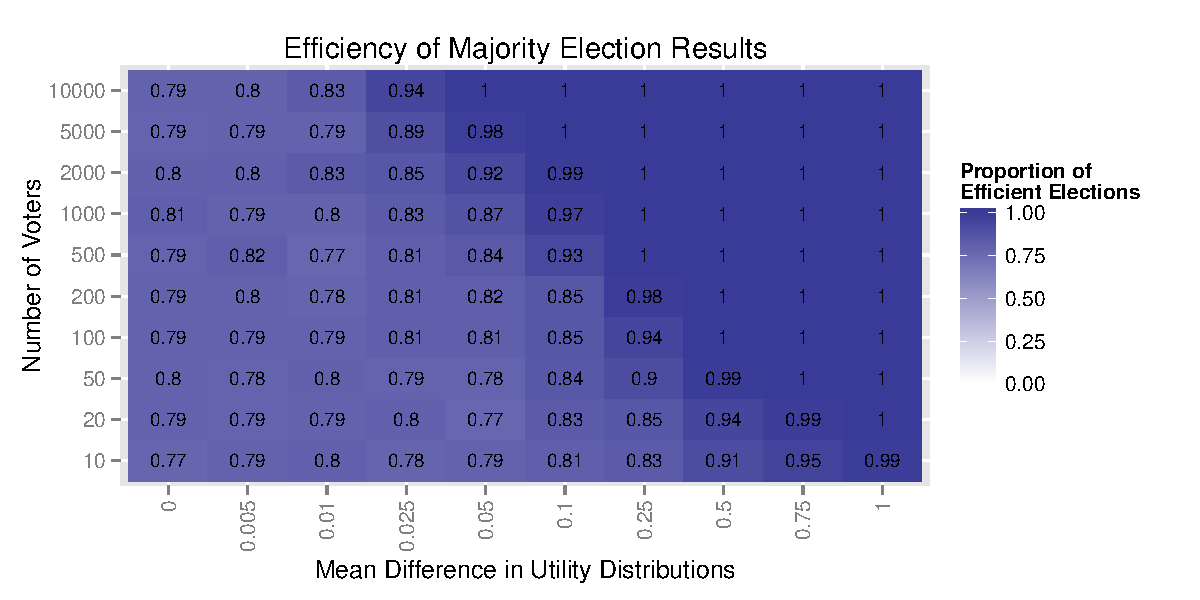
\includegraphics[height=.7\textheight]{../calc/fig/s3b.pdf}
  \end{figure}
  $$U^a_i \sim \mathcal{N}(\mu=0,\sigma^2=1) \hspace{1cm}
  U^b_i \sim \mathcal{N}(\mu=0+\epsilon,\sigma^2=1)$$
\end{frame}

\subsection{}
\begin{frame}%[allowframebreaks]
  \frametitle{Investigating the effect of skewed utility distributions I}
  \begin{figure}[ht]\centering
    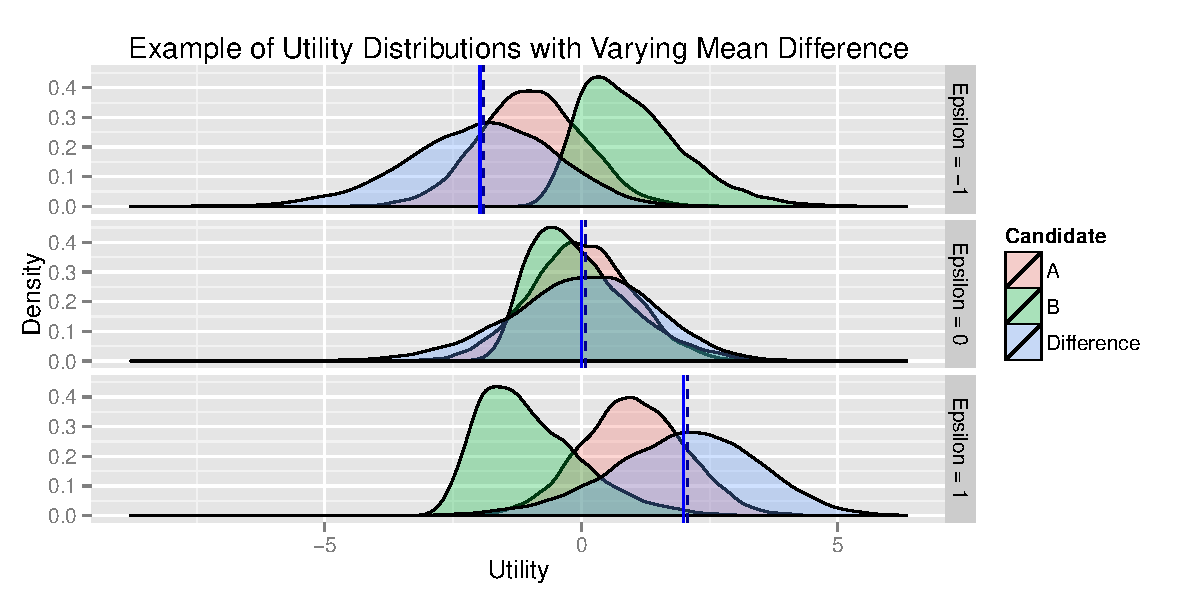
\includegraphics[height=.7\textheight]{../calc/fig/s4a.pdf}
  \end{figure}
  $$U^a_i \sim \mathcal{N}(\mu=0+\epsilon,\sigma^2=1) \hspace{1cm}
  U^b_i \sim \mathcal{N}_\text{skew}(\mu=0-\epsilon,\sigma^2=1)$$
\end{frame}
\begin{frame}%[allowframebreaks]
  \frametitle{Investigating the effect of skewed utility distributions II}
  \begin{figure}[ht]\centering
    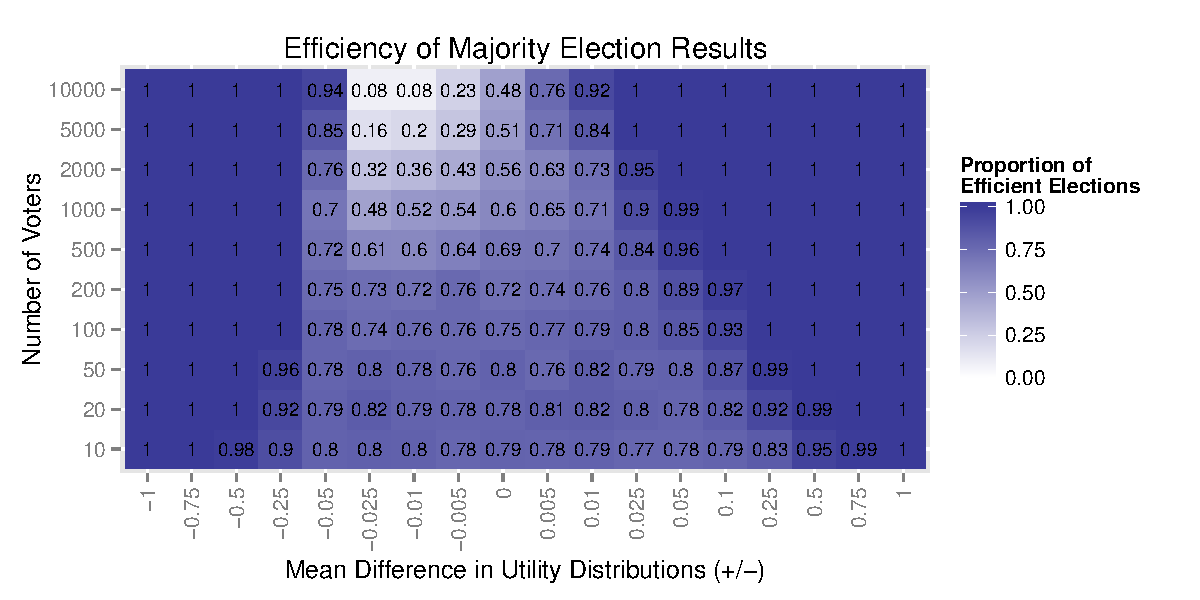
\includegraphics[height=.7\textheight]{../calc/fig/s4b.pdf}
  \end{figure}
  $$U^a_i \sim \mathcal{N}(\mu=0+\epsilon,\sigma^2=1) \hspace{1cm}
  U^b_i \sim \mathcal{N}_\text{skew}(\mu=0-\epsilon,\sigma^2=1)$$
\end{frame}

\section{Discussion and Experimental Designs}
\subsection{}
\begin{frame}%[allowframebreaks]
  \frametitle{Discussion of Results}
  \begin{itemize}
    \item \emph{Relaxing assumptions} about ideal-point based preferences can reduce the likelihood that election results are efficient
    \begin{itemize}
      \item \emph{mean difference} and \emph{skewness} of the distributions of individual utilities for each candidate affects the likelihood of inefficiencies
      \item under some scenarios, increasing the \emph{size of the electorate} actually reduces the efficiency of majority voting!
    \end{itemize}
    \item \emph{Question}: conceptualization of utility reasonable? These results would not hold if preferences were purely ordinal (and utilities not comparable across individuals)
  \end{itemize}
\end{frame}

\subsection{}
\begin{frame}%[allowframebreaks]
  \frametitle{Possible Experimental Designs and Further Developments}
  \begin{itemize}
    \item Performance of \emph{compensation elections / bidding mechanisms} in the context of binary choices \citep{oprea2007compensation}
    \item Effect of (endogenous) electoral \emph{abstention} on election efficiency
    \item Multi-candidate elections
  \end{itemize}
\end{frame}

\subsection{}
\begin{frame}
  \frametitle{References}
  \def\newblock{\hskip .11em plus .33em minus .07em}
  %\nocite{*}
  \begin{scriptsize}
    \bibliographystyle{apsr}
    \bibliography{/data/Dropbox/1-src/lit/Literature}
  \end{scriptsize}
\end{frame}

\section{Appendix}
\subsection{}
\begin{frame}%[allowframebreaks]
  \frametitle{Inducing inefficiencies with ideal point utilities I}
  \begin{figure}[ht]\centering
    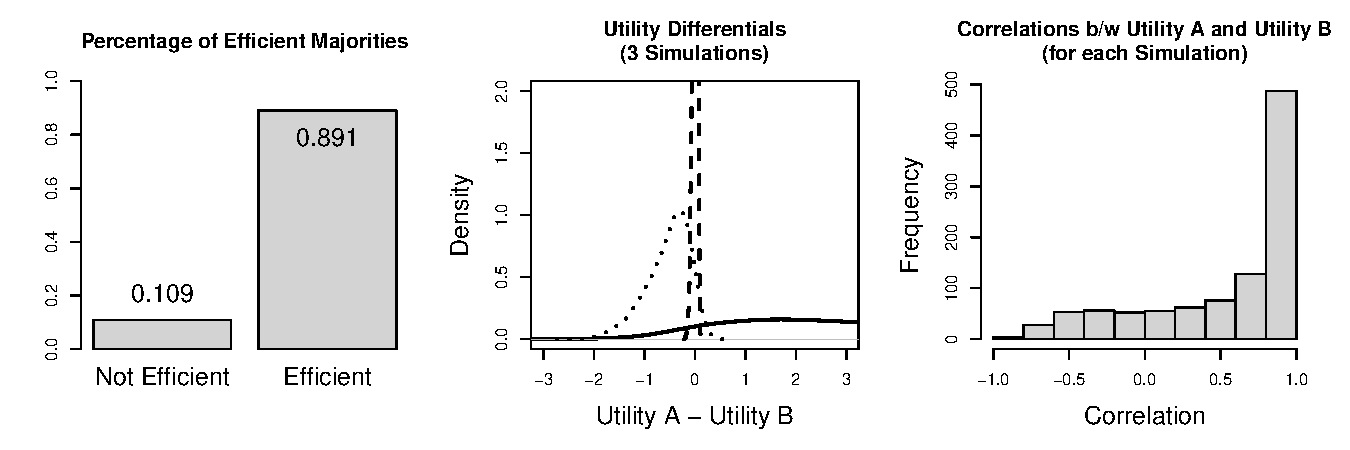
\includegraphics[width=\textwidth]{../calc/fig/sX1.pdf}
    \caption{Skewed ideal points}
  \end{figure}
  $$X_i \sim \mathcal{N}_\text{skew}(\mu=0,\sigma^2=1) \hspace{1cm} X_a,X_b \sim \mathcal{N}(\mu=0,\sigma^2=1)$$
  $$U^a_i = -(X_i - X_a)^2 \hspace{1cm} U^b_i = -(X_i - X_b)^2$$
\end{frame}
\subsection{}
\begin{frame}%[allowframebreaks]
  \frametitle{Inducing inefficiencies with ideal point utilities II}
  \begin{figure}[ht]\centering
    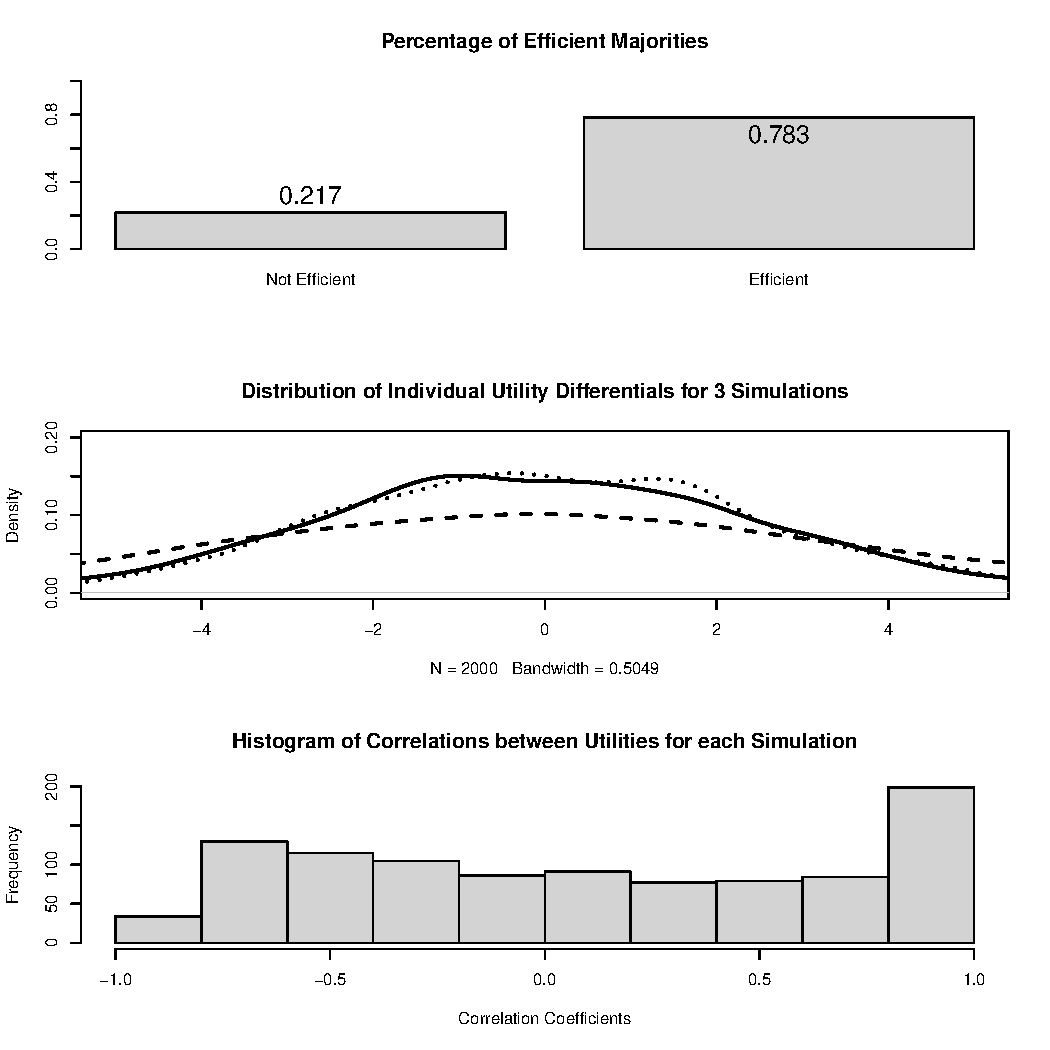
\includegraphics[width=\textwidth]{../calc/fig/sX2.pdf}
    \caption{Aggregate indifference between ideal points}
  \end{figure}
  $$X_i,X_a \sim \mathcal{N}(\mu=0,\sigma^2=1) \hspace{1.4cm} X_b = -1*X_a $$
  $$U^a_i = -(X_i - X_a)^2 \hspace{2cm} U^b_i = -(X_i - X_b)^2$$
\end{frame}


\end{document}